  
% ------------------------
% DB and Confidence Science Manuscript
% ------------------------

%\documentclass{nature,floatsintext}


\documentclass[a4paper,doc,natbib,floatsintext]{apa6}
\usepackage[english]{babel}
\usepackage[utf8x]{inputenc}
\usepackage{amsmath}
\usepackage{graphicx}
\usepackage{rotating}
\usepackage{pdfpages}
%\usepackage{Sweave}
\usepackage{subcaption}
\usepackage{float}

\title{Peeks and Keeps: A new paradigm for studying the exploration-exploitation trade-off}
\shorttitle{Peeks and Keeps}
\twoauthors{Nathaniel D. Phillips and Hans Joerg Neth}{Daniel Navarro}
\twoaffiliations{University of Konstanz}{University of Adelaide}

\abstract{Many important decision tasks involve an exploration-exploitation trade-off, where organisms have the competing goals of gaining new information (exploration) to improve future decisions, and acting on existing information (exploitation). The most common paradigm to study this trade-off experimentally is the n-armed bandit, where decision makers reap real costs and rewards on every trial. We suggest that, unlike the n-armed bandit, many real world tasks allow decision makers to explore options (such as stock price changes) without reaping any costs or rewards. To address this, we introduce a new experimental paradigm called ``Peeks and Keeps'' that combines aspects of the n-armed bandit with the `bet-observe' task \citep{tversky1966information}. Unlike the n-armed bandit, Peeks and Keeps gives decision makers the option of explicitly separating exploration and exploitation behavior, where exploration provides only information but no costs or rewards, and exploitation gives both information and costs and rewards. This paradigm not only increases the empirical validity of the n-armed bandit, but also provides researchers with an explicit measure of exploration that is hidden in other paradigms.}

\keywords{exploration, exploitation, decisions from experience, decisions under uncertainty}


\begin{document}

\begin{knitrout}
\definecolor{shadecolor}{rgb}{0.969, 0.969, 0.969}\color{fgcolor}\begin{kframe}
\begin{alltt}
\hlkwd{setwd}\hlstd{(}\hlkwc{dir} \hlstd{=} \hlstr{"/Users/Nathaniel/Dropbox/Git/PeeksAndKeeps"}\hlstd{)}

\hlstd{mcmc.samples} \hlkwb{<-} \hlnum{1000}
\hlstd{mcmc.burnin} \hlkwb{<-} \hlnum{10}
\end{alltt}
\end{kframe}
\end{knitrout}



\maketitle

\section*{Introduction}

\subsection{Exploration-exploitation trade-off}

Many of the most important real world decisions require individuals to reap consequences from several risky options that probabilistically give rewards and punishments. In many tasks, these decisions are made under uncertainty, where the probabilities and magnitudes associated with options are \textit{a priori} unknown. In order to learn about options, organisms can engage in active search which improves the quality of their impressions of options. However, search can come at a cost, such as the missed opportunity to receive rewards from known options. For example, in trying a new restaurant, one forgoes the opportunity to have a meal at her (current) favorite restaurant.

This conflict between obtaining new information and acting on existing information is known as the exploration-exploitation trade-off. The exploration-exploitation (EE) trade-off is one of the most widely studied aspects of decision making from human to non-human organisms. The exploration-exploitation trade-off represents a goal conflict in decisions under uncertainty, where an organism is trying to maximize its long term rewards from \textit{a priori} unknown options. On the one hand, individuals want to explore options by gaining as much information as possible to improve the quality of their future decisions. On the other hand, they want to \textit{exploit} options by acting on existing information in order to increase short-term rewards.

One of the most widely used experimental tasks used to study the exploration-exploitation conflict is the n-armed bandit. In an n-armed bandit, participants have a fixed number of trials to select an option and experience a consequential reward.




\subsection{Purely epistemic versus pragmatic actions}

\begin{itemize}

  \item \cite{neth2008thinking} distinguished between two types of actions, epistemic and pragmatic. Epistemic actions are those that result in information rather than punishments or rewards, while pragmatic actions are those that lead to punishments or rewards. Exploration is assumed to be an epistemic action while exploitation is a pragmatic action.
  
  \item One can easily imagine real-world cases where people explicitly engage in purely epistemic actions. For example, imagine a person who wishes to learn about the stock market prior to risking any real money. He can do this by viewing sequential returns from several stocks and observing their risk. Alternatively, a new resident to a town can learn about local restaurants by asking her neighbors about their recent experiences. In all of these cases, the actor is learning about options without reaping consequences.
  
  \item Clearly these purely epistemic actions are both psychologically and behaviorally distinct from pragmatic actions, where one obtains \textit{both} information and immediate consequences. For example, our stock investor who starts investing his money into stocks will then not only learn about their performance, but also reap gains and suffer consequences. Similarly, the new town resident who starts frequenting local restaurants will continue learning about them but also experience immediate pragmatic outcomes.
  
  \item Somewhat puzzlingly, paradigms that have been used to study exploration-exploitation trade-off in humans has largely ignored behavioral differences in epistimic and pragmatic actions. In the N-armed bandit task, players are only allowed to engage in one type of behavior - choice, which always provides both epistemic and pragmatic rewards. Players are not given the option to engage in purely epistemic actions. 
  
  \item This can lead to erroneous inferences. The same choice behavior could be interpreted as either resulting from an epistemic or pragmatic motivation. Until now, researchers have had to use computational cognitive modeling techniques to attribute choices post-hoc to either an epistemic or pragmatic underlying goal.
  
  \item We believe a new paradigm is needed. One where individuals have the option to explicitly explore or exploit options. This task will not only be a better model of many real-world decision tasks than previous paradigms, but will also allow researchers to explicitly observe behavior consistent with purely epistemic goals.

\end{itemize}

\subsection{Combining three paradigms}


\begin{center}
    \begin{tabular}{ | l | l | l | l | l |}
    \hline
    Paradigm & EE Tradeoff & Pure Exploration & Pure Exploitation & Alternation \\ \hline
    N-Armed Bandit & Yes & No & No & Yes\\ \hline
    Sampling Paradigm & No & Yes & Yes & No\\ \hline
    Bet-Observe & Yes & Yes & Yes & Yes\\ \hline
    Peeks and Keeps & Yes & Yes & No & Yes\\ \hline
    \hline
    \end{tabular}
\end{center}


In a multi-armed bandit task, participants choose between multiple a priori unknown options over several trials and receive rewards (or costs) on each trial. Because decision makers reap consequences on every trial, the n-armed bandit task does not allow purely epidemic actions. The Iowa Gambling Task (IGT) is one famous example of this paradigm. Using cognitive models such as the expectancy-valence model, researchers have used the IGT to study cognitive mechanisms such as loss-aversion, recency, and choice consistency in both healthy and non-healthy individuals \citep{yechiam2005models}.

Two paradigms have been used to study purely epistemic actions: the sampling paradigm of decisions from experience \citep{hertwig2004decisions} and the bet-observe task \citep{tversky1966information}. Like the n-armed bandit task, both paradigms present participants with multiple, a priori unknown options. In the sampling paradigm, participants can then sample from options, without consequence, as many times as they would like before making a single consequential choice. Here, participants engage in a self-determined number of purely epistemic actions strictly prior to a single purely pragmatic action. After making their final choice, participants receive the consequences from their choice but cannot continue to observe. Thus, in the sampling paradigm observation strictly occurs prior to exploitation with no possibility to alternate between the two modes.

As far as we know, the bet-observe task is the only paradigm that allows individuals to alternate between pure exploration and pure exploitation. In the bet-observe task, an individual is presented with two options. On each of M trials, one of the two options will produce a reward indicated by a green light. On each trial, the participant selects an option and makes one of two choices. He can \textit{observe} an option, see which one produces the reward, but not receive the reward. Or he can \textit{bet} on an option. If the player bets on an option, he will gain its underlying reward but will not see whether the reward is present. Because the participant only sees the option outcome if he observes, he can only learn about the options' underlying distributions on observation trials, but can only reap rewards on betting trials.

Navarro and Newell (2014) derived optimal decision strategies for two versions of the game: stationary and non-stationary. In the stationary version of the game, the reward probability distributions are fixed. Specifically, the probability that the left option has a reward $l_{p}$ is fixed and does not change over time. In the stationary task, an optimal learner will begin the task by observing outcomes until he reaches a pre-defined information threshold. Once he reaches this threshold, he will switch to a betting strategy and will always bet on the perceived better option. In the non stationary version of the game, the reward probability distributions can change at any time. For example, with some probability $\alpha$ the probability $l_{p}$ could change to a value drawn from a uniform distribution. In this version of the game, the optimal decision strategy alternates between observing and betting throughout the game. In other words, the actor will begin by observing for a few trials until a certain information threshold is reached, then he will switch to betting for a few trials. He will then switch to observing in order to see if $l_{p}$ has changed.

However, because betting in the bet-observe task does not provide information, decision makers cannot learn anything on betting trials. This is not an inherent flaw in the paradigm - indeed, obscuring information from betting trials elegantly separates epistemic from pragmatic actions. However, because many, if not most, real-world decision tasks provide information on both exploration and exploitation trials, the bet-observe task is a poor model of most real-world decisions. From food choice to mate choice, exploitation decisions (i.e.; consuming food or selecting a mate) will always provide information to the decision maker that it can use to update its impressions and guide future search. 

In order to study how people alternate between explicit exploration and exploitation, we introduce the Peeks and Keeps task.


\section{Peeks and Keeps}

Peeks and Keeps is an extension of an N-armed bandit task that explicitly separates exploration and exploitation decisions. In the task, participants repeatedly select one of N options with \textit{a priori} unknown underlying probability distributions over the course of M trials. On each trial, the participant selects an option and elects to either \textit{observe} the next outcome without financial feedback, or \textit{bet} on the outcome and receive the financial feedback. At the end of M trials, the participant is paid the sum of all sample outcomes revealed on bet trials. If he always observes and never bets, he receives no bonus. If he bets on every trial, he receives the sum total of all samples.



\section{``Optimal'' Search in Peeks and Keeps}

How many peeks \textit{should} people take when playing peeks and keeps? The answer to this question depends on two critical criteria: the specific search strategy a person uses, and the statistical environment they are in. To reduce the strategy and environmental space, we will make several restrictions. 

With regard to search strategies, we assume that people use a simple ``explore equally then exploit'' strategy. This strategy assumes that people begin by exploring the environment using a pre-defined number of peeks - where the exact number of peeks varies across agents. Once the person has used all of their peeks, they shift to a soft-max exploitation strategy.

With regard to environments, we assume that each environment has three stable options. Thus, environments are static.

In Figure XXX, we plot the environments and the median number of points earned by 5,000 agents using 0 to 100 peeks:

% Optimal Peeks Simulation


% Plot optimal peeks simulation


We begin with environment 1. This environment has a negative (mean = -5), neutral (mean = 0) and positive (mean = +5) option, and each option has a relatively small standard deviation of 5. Here, the optimal number of peeks is just 0, suggesting that the environment is so easy to learn that the opportunity costs of peeking outweigh the benefits. Environment 2 takes the same options from Environment 1, but increases the standard deviation of options from 5 to 30. Here, learning should be more difficult and potentially increase the benefits of peeking. Consistent with this prediction, we find that the optimal number of peeks in Environment 2 is 20.



% Custom Functions


% Load Datafiles


% Create dataframes
\begin{knitrout}
\definecolor{shadecolor}{rgb}{0.969, 0.969, 0.969}\color{fgcolor}\begin{kframe}
\begin{verbatim}
## NULL
\end{verbatim}
\end{kframe}
\end{knitrout}








\section{Method}

\subsection{Participants}

Participants (N = 250) were recruited from the Amazon Mechanical Turk\footnote{We restricted our study to workers who had completed at least 100 HITs with at least a 95\% HIT acceptance rate.}. For their paritcipation, workers received a guaranteed reward of 50 cents with the possibility of a bonus up to \$1.00. 122 (49\%) were female and the mean age was (35.66) (IQR: [27, 42])

\subsection{Procedure}

We created 6 sequences of 200 integers following a rounded Normal distribution with means of -5, 0 or +5 (corresponding to the positive, neutral, and negative options) and standard deviation of 10 or 30 (corresponding to the easy and difficult distributions)\footnote{In order to ensure that the sample distributions closely matched the desired means and standard deviations, we repeatedly generated candidate sample distributions until we found ones whose sample means were within 0.10 of the desired mean and whose standard deviations were within 1.0 of the desired value. Additionally, we truncated the distributions so the minimum and maximum values did not exceed -99 and +99 respectively.}. In the \textit{dynamic} condition, the location of the positive and negative options changed places on trial 101, while in the \textit{stable} condition there was no change. To prevent any option order counfounds, we employed all 6 possible orderings of the options on the screen as a between-subjects factor. However, for all of our analyses we have ignored this factor.

Each participant was randomly assigned to one of the 48 conditions (Response Mode (Peeks vs. Keeps) x Stimuli Difficulty (Easy vs. Hard) x Environment Stability (Stable vs. Dynamic) x Option Order). In both response mode conditions, participants were told that the goal of the game was to earn as many points as possible over the course of 200 trials using their 200 Keeps (for the Keeps condition) or their 200 Peeks and Keeps (for the Peeks condition). To reinforce the idea that peeking introduces an opportunity cost, Those in the Peeks condition were specifically told that using a Peek action would `use a trial.' Participants were not explicitly told that the options would be either stable or dynamic. Instead, all participants were told that at any given point in the game, one of the options would be the best one.

After completing all 200 trials, participants completed three personality questionnaires (the XX, YYY, and the ZZZ) and an additional post-study questionnaire that elicited their overall impressions of the game.

\section{Results}

\subsection{Point Totals}

\begin{figure}
\centering
\begin{knitrout}
\definecolor{shadecolor}{rgb}{0.969, 0.969, 0.969}\color{fgcolor}
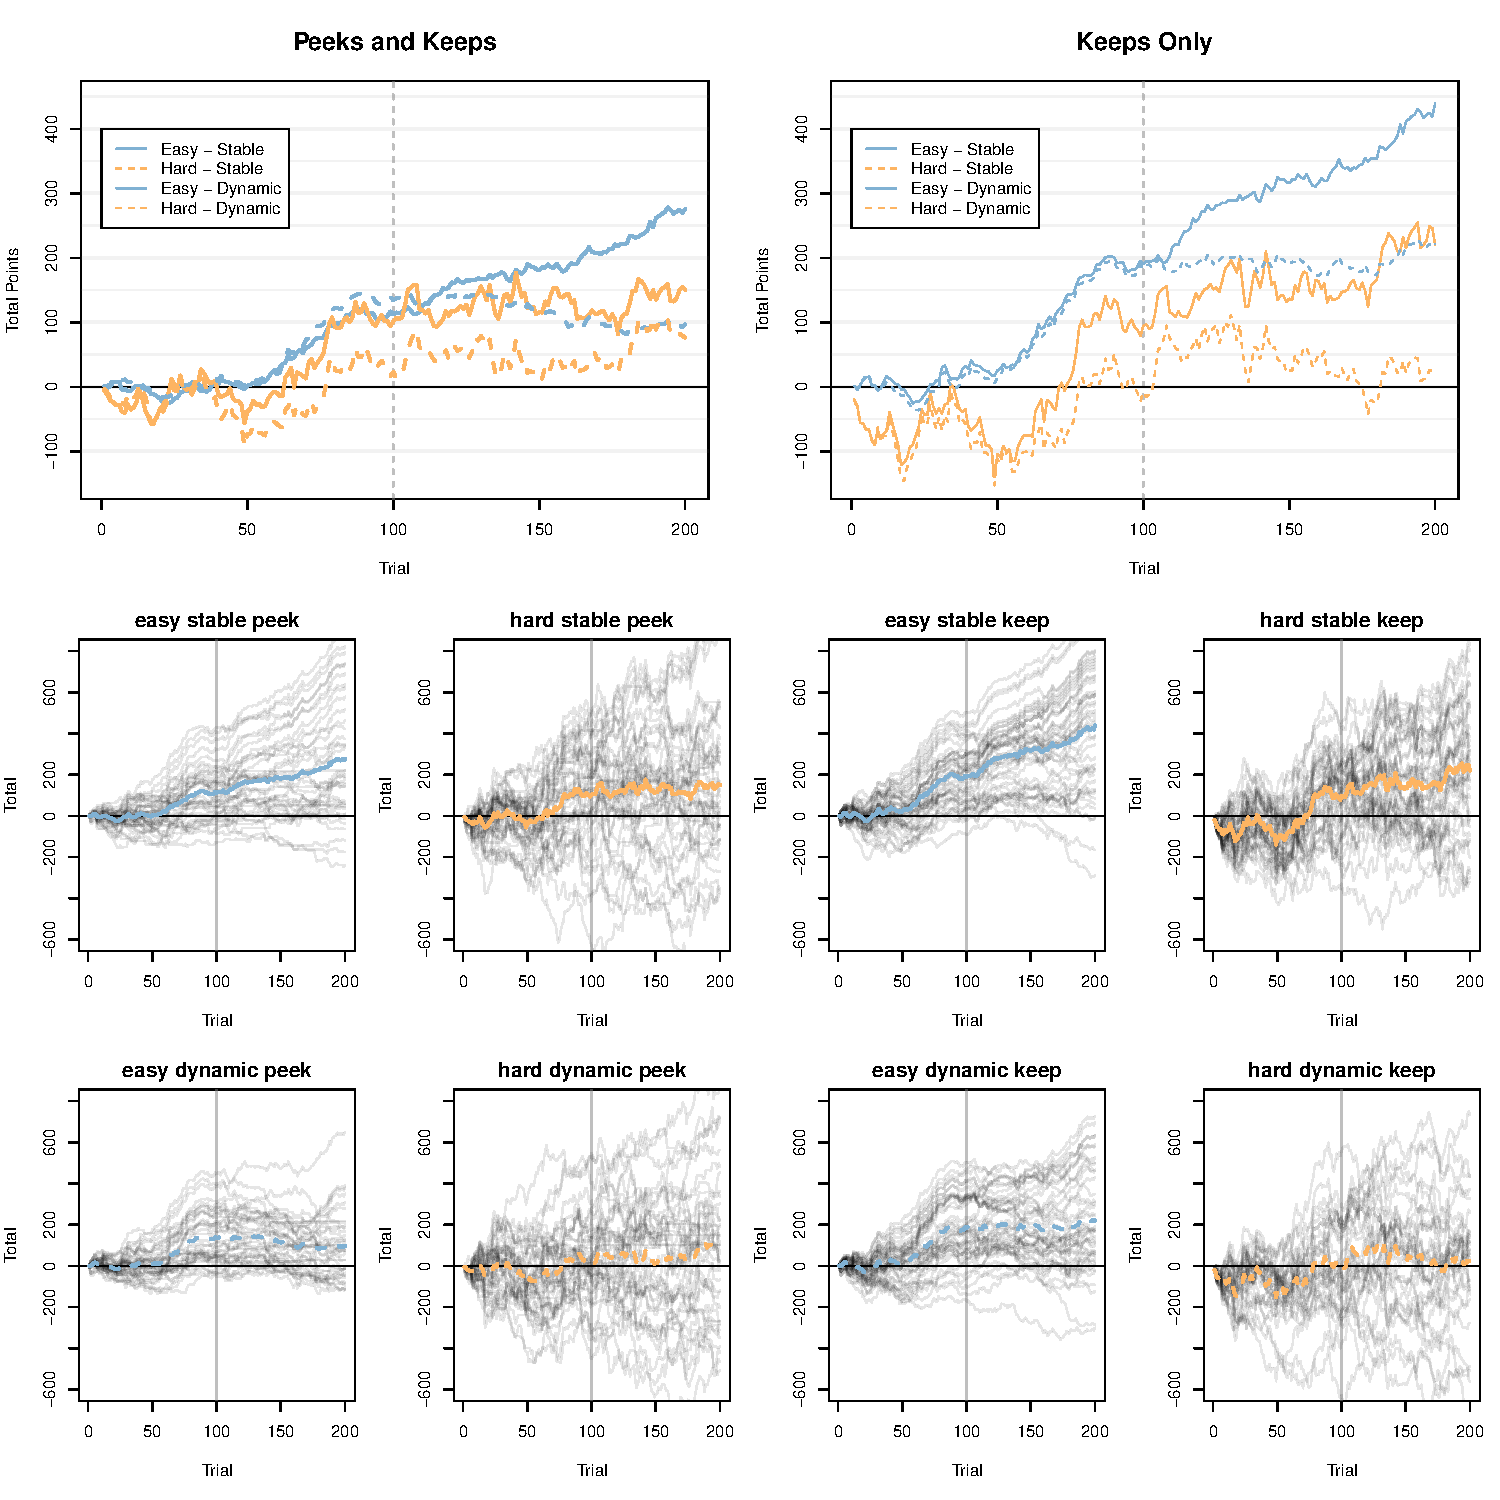
\includegraphics[width=\maxwidth]{figure/unnamed-chunk-9-1} 

\end{knitrout}
\caption{\label{fig:pointsbytrial}Cumulative point tradjectories across trials for all conditions and participants. The two panels in the top row show the average cumulative point values across participants for each experimental condition. The bottom 8 plots in the bottom two rows show the mean tradjectory of each condition separately, with individual lines plotted for each individual participant.}
\end{figure}


Summary statistics of the cumulative point totals earned by participants in each of the experimental conditions are shown in Table~\ref{table:MeasuresTbl}. Additionally, group mean and individual level cumulative point values across trials are shown in Figure~/ref{fig:pointsbytrial}. To see which experimental variables affected point totals, we conducted a Bayesian regression analysis with each participant's point total as the dependent variable and the three experimental conditions as independent variables. Results are shown in Table~\ref{table:totals.model}. We found a credible negative effect of the difficult stimuli condition for both trials 1-100 and trials 101-200, suggesting that participants did worse in the difficult environment than the easy environment. For trials 101-200 we found that participants in the dynamic condition performed credibly worse than those in the stable condition.

% Regression model HDIs


















